%%----------------------------------------------------------------------------
%% Presentatie HoGent Bedrijf en Organisatie
%%----------------------------------------------------------------------------
%% Auteur: Bert Van Vreckem [bert.vanvreckem@hogent.be]

\documentclass{beamer}

%==============================================================================
% Aanloop
%==============================================================================

%---------- Packages ----------------------------------------------------------

\usepackage{graphicx,multicol}
\usepackage{comment,enumerate,hyperref}
\usepackage{amsmath,amsfonts,amssymb}
\usepackage{tikz}
\usepackage{lmodern}
\usepackage[T1]{fontenc}
\usepackage[utf8]{inputenc}
\usepackage{csquotes}
\usepackage[english]{babel}
\usepackage{multirow}
\usepackage{eurosym}
\usepackage{listings}
\usepackage{textcomp}
\usepackage{framed}
\usepackage{wrapfig}
\usepackage[backend=biber,style=apa]{biblatex}
\DeclareLanguageMapping{english}{english-apa}
\addbibresource{research-techniques-ex1.bib}

%---------- Configuratie ------------------------------------------------------

\usetikzlibrary{arrows,shapes,backgrounds,positioning,shadows}

\usetheme{hogent}

%---------- Commando-definities -----------------------------------------------

\newcommand{\tabitem}{~~\llap{\textbullet}~~}

%---------- Info over de presentatie ------------------------------------------

\title[Intro]{Research techniques\\Seminar session 1. \LaTeX{}}
\author{Anita Bernard, Jens Buysse, Bert {Van Vreckem}}
\date{AY 2016-2017}

%==============================================================================
% Inhoud presentatie
%==============================================================================

\begin{document}

%---------- Front matter ------------------------------------------------------

% Dia met het HoGent logo
\HoGentLogo

% Titeldia met faculteitslogo
\titleframe

%---------- Inhoud ------------------------------------------------------------

\begin{frame}
  \frametitle{What's on the menu today?}

  \tableofcontents
\end{frame}

\section{Introduction}

\subsection{Philosophy, history}

\begin{frame}
  \frametitle{Pholosophy: why {\LaTeX}?}
  
  \begin{itemize}
  \item<+-> WYSIWYG text processors force authors to do layout
  \item<+-> Consequence: ugly, inconsistent documents
  \item<+-> A professional layout is a specialty and should not be left to authors.
  \item<+-> Ambition of {\LaTeX} is to allow authors to only worry about \emph{content} and \emph{structure}
  \end{itemize}
\end{frame}

\begin{frame}
  \frametitle{History}

  \begin{columns}[c]

  \column{.67\textwidth}
    \begin{itemize}
    \item<+-> 1977: Donald Knuth receives galley proofs of his book \emph{The art of Computer Programming} awful
    \item<+-> 1978: Started writing his own typesetting system, {\TeX}
    \item<+-> 1989: Version 3.0, only bugfix-releases since then (converge to $\pi$)
    \item<+-> 1980s: Leslie Lamport develops a markup language for {\TeX}: {\LaTeX}
    \end{itemize}

  \column{.33\textwidth}
    \begin{center}
    \only<1-3>{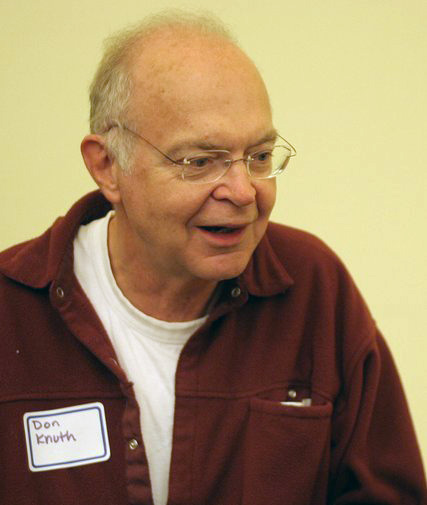
\includegraphics[width=\textwidth]{img/oef1-01}}
    \only<4->{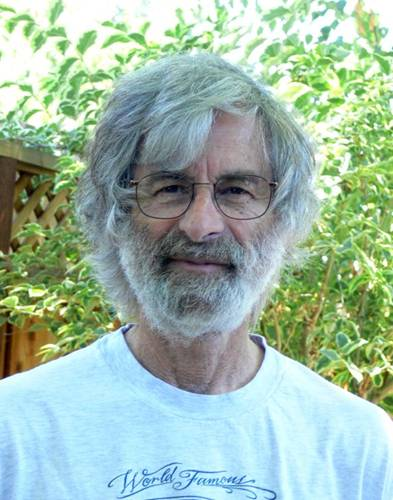
\includegraphics[width=\textwidth]{img/oef1-02}}
    \end{center}

  \end{columns}
\end{frame}

\subsection{Examples}

\begin{frame}
  \frametitle{Examples---papers}

  {\LaTeX} is the standard format for scientific publications in computer science, mathematics, physics, etc.

  \begin{center}
  
\includegraphics[height=.6\textheight]{img/oef1-03}
  \end{center}

\end{frame}

\begin{frame}
  \frametitle{Examples---books}

  Also: courses, thesisses, etc.

  \begin{center}
	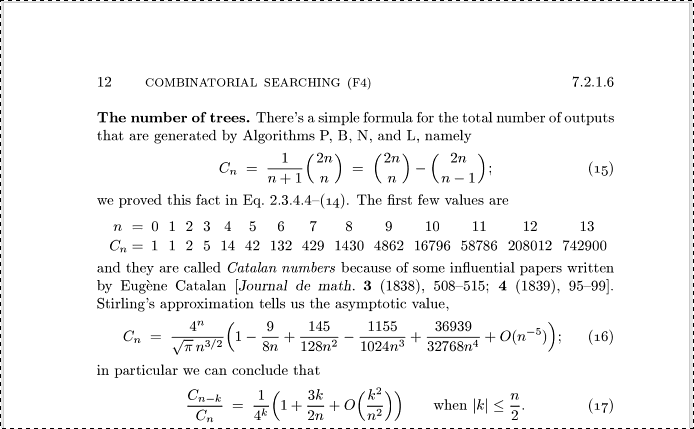
\includegraphics[height=.6\textheight]{img/oef1-04}
  \end{center}

\end{frame}

\begin{frame}
  \frametitle{Examples---presentation slides}

  \begin{center}
  e.g.~this presentation\ldots
  \end{center}

\end{frame}

\begin{frame}
  \frametitle{Advantages}

  \begin{itemize}
    \item<+-> Focus on contents, a professional layout is guaranteed.
    \item<+-> Text-based format $\Rightarrow$ suitable for a version control system!
    \item<+-> Standard format in several research domains, a.o.~computer science.
  \end{itemize}
\end{frame}


\begin{frame}
  \frametitle{Disadvantages}

  \begin{itemize}
    \item<+-> Steep learning curve. Copy/paste examples, look it up, ask for help.
    \item<+-> Sometimes, the desired layout can't be obtained easily (e.g.~tables)
  \end{itemize}

  \uncover<1->{%
    \begin{center}
      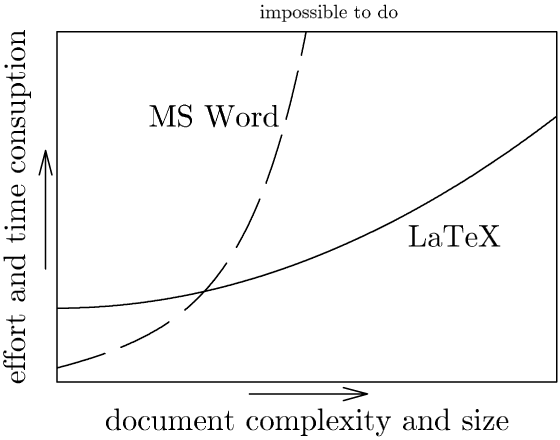
\includegraphics[height=.5\textheight]{img/oef1-05}
    \end{center}}
\end{frame}

\subsection{Finding help}

\begin{frame}
  \frametitle{Finding help}

  \begin{itemize}
  \item Tobias Oetiker, et al., \emph{The Not So Short Introduction to {\LaTeXe}}, 2011 (a.k.a. ``lshort'', version 5.01)
  \item {\TeX} - {\LaTeX} StackExchange (Q \& A site): \url{http://tex.stackexchange.com/}
  \item \emph{{\LaTeX} Wikibook}, \url{http://en.wikibooks.org/wiki/LaTeX}
  \item \emph{Hypertext help with {\LaTeX}}, \url{http://www.ics.uci.edu/~pan/documents/latex/ltx-2.html}
  \end{itemize}

\end{frame}

\section{Getting started with {\LaTeX}}

\subsection{Set up environment}

\begin{frame}
  \frametitle{Set up environment}

(1) {\LaTeX} distribution

  \begin{itemize}
  \item Windows: MikTeX \url{http://miktex.org/}
  \item MacOS: MacTeX distribution \url{http://www.tug.org/mactex/2011/}
  \item Linux: available out of the box
    \begin{itemize}
    \item Ubuntu, Debian: \texttt{sudo apt-get install texlive}
    \item Fedora: \texttt{sudo dnf install texlive}
    \end{itemize}
  \item On-line editor: \url{https://www.overleaf.com/}
  \end{itemize}

(2) {\LaTeX} editor

  \begin{itemize}
  \item Several choices, depending on the operating system
  \item e.g. TexStudio \url{http://www.texstudio.org/}
  \end{itemize}
\end{frame}

\subsection{Document structure}

\begin{frame}
  \frametitle{Workflow}

  \begin{itemize}
  \item<+-> Write the text in {\LaTeX}
  \item<+-> Compile the file (with e.g.~\texttt{pdflatex} or \texttt{latexmk})
  \item<+-> View result in PDF viewer
  \end{itemize}
\end{frame}

\begin{frame}[fragile]
  \frametitle{{\LaTeX} commands}

  \begin{block}{Basic syntax}
  \verb|\command[optional,arguments]{arg1}{arg2}|
  \end{block}

  \pause

  Example:

  \begin{itemize}
  \item<+-> \verb|\documentclass[a4paper,pdftex,12pt]{paper}|
  \item<+-> \verb|\'{e}l\`{e}ve| $\Rightarrow$ \'el\`eve
  \item<+-> \verb|\begin{itemize}|\\
            \verb|\item list|\\
            \verb|\end{itemize}|
  \end{itemize}

\end{frame}

\begin{frame}[fragile]
  \frametitle{Structure of a document}
  
  \begin{center}
  \alert{%
  \only<1>{Define document type (here: article)}
  \only<2>{``body'' of the document}
  \only<3>{Document content}
  \only<4>{Activate extra functionality}
  \only<5>{Title, author are specified in ``preamble''}
  \only<6>{Add title into the document}
  }
  \end{center}

\begin{semiverbatim}
\uncover<1->{\alert<1>{\\documentclass[a4paper,12pt]\{article\}}}
\uncover<4->{\alert<4>{\\usepackage[dutch]\{babel\}}}
\uncover<5->{\alert<5>{\\title\{Minimaal \{\\LaTeX\} document\}}}
\uncover<5->{\alert<5>{\\author\{Bert \{Van Vreckem\}\}}}
\uncover<5->{\alert<5>{\\date\{\\today\}}}
\uncover<2->{\alert<2>{\\begin\{document\}}}
\uncover<6->{\alert<6>{\\maketitle}}
\uncover<3->{\alert<3>{Lorem ipsum dolor sit amet, consectetur adipiscing elit.}}
\uncover<2->{\alert<2>{\\end\{document\}}}
\end{semiverbatim}

\end{frame}

\begin{frame}
  \frametitle{Result}
  
  \begin{center}
  
\includegraphics[height=.6\textheight]{img/oef1-06}
  \end{center}
\end{frame}

\begin{frame}[fragile]
  \frametitle{Document types}
  
  \begin{center}
  \begin{semiverbatim}
  \\documentclass[\alert<2>{OPTIONS}]\{\alert<1>{TYPE}\}
  \end{semiverbatim}
  \end{center}

\only<1>{%  
  \begin{center}
  \begin{tabular}{ll}
    \hline
    TYPE & document type \\
    \hline
    \texttt{article} & article, paper, short text \\
    \texttt{beamer} & presentation \\
    \texttt{book} & book \\
    \texttt{report} & (long) report, thesis, \ldots \\
  \end{tabular}
  \end{center}
}
\only<2>{%  
  \begin{center}
  \begin{tabular}{ll}
    \hline
    OPTION & effect \\
    \hline
    \texttt{12pt} & 12-point letters (instead of 10pt) \\
    \texttt{a4paper} & A4 (instead of Am. Letter) \\
    \texttt{twocolumn} & customary for articles \\
    \texttt{twoside} & two side printing (larger inner margins) \\
  \end{tabular}
  \end{center}
}
\end{frame}



\begin{frame}[fragile]
  \frametitle{Document structure}
  
  \begin{center}
  \begin{tabular}{ll}
    \verb?\part? & (no influence on chapter numbers) \\
    \verb?\chapter? & (only in \texttt{book}, \texttt{report}) \\
    \verb?\section? & \\
    \verb?\subsection? & \\
    \verb?\subsubsection? & (not in \texttt{book}, \texttt{report}) \\ 
    \verb?\paragraph? & \\
    \verb?\subparagraph? & \\
    &\\
    \verb?\appendix? & from this point \verb?\chapter? becomes an Appendix \\
    \verb?\label{?\texttt{\ldots}\verb?}? & for references (with \verb|\ref{LABEL}|)
  \end{tabular}
  \end{center}
\end{frame}

\begin{frame}[fragile]
  \frametitle{Preamble---Useful packages}
  
  \begin{description}
  \item[\texttt{\textbackslash{}usepackage\{amsfonts\}}] AMS math packages: extra mathematical
  \item[\texttt{\textbackslash{}usepackage\{amsmath\}}] symbols (a.o. number sets
  \item[\texttt{\textbackslash{}usepackage\{amssymb\}}] $\mathbb{N}, \mathbb{R}, \mathbb{Z}, \mathbb{Q}$, etc.)
  \pause
  \item[\texttt{\textbackslash{}usepackage[dutch]\{babel\}}] Language settings: hyphenation, special characters
  \pause
  \item[\texttt{\textbackslash{}usepackage\{eurosym\}}] Euro-symbol (\euro)
  \pause
  \item[\texttt{\textbackslash{}usepackage\{fancyhdr\}}] Page layout with header and footer
  \pause
  \item[\texttt{\textbackslash{}usepackage\{graphicx\}}] Inserting figures
  \end{description}
\end{frame}

\begin{frame}[fragile]
  \frametitle{Preamble---Useful packages}
  
  \begin{description}
  \item[\texttt{\textbackslash{}usepackage[pdftex,bookmarks=true]\{hyperref\}}] clickable links in PDF for table of contents, etc. \pause
  \item[\texttt{\textbackslash{}usepackage[utf8]\{inputenc\}}] Use accented characters in the source text (e.g. é ipv \verb|\'e|) \pause
  \item[\texttt{\textbackslash{}usepackage\{listings\}}] Source code\pause
  \item[\texttt{\textbackslash{}usepackage\{multirow\}}] Merge cells in tables\pause
  \item[\texttt{\textbackslash{}usepackage\{rotating\}}] Rotate figures and tables \pause
  \item[\texttt{\textbackslash{}usepackage\{lipsum\}}] Filler text (lorem ipsum dolor sit amet\ldots)
  \end{description}
\end{frame}

\subsection{Writing {\LaTeX}}

\begin{frame}[fragile]
  \frametitle{Special characters}
  
  \begin{itemize}
  \item<+-> Special characters ({\LaTeX} syntax): \% \$ \& \{ \} \textbackslash{} enz: \\
\begin{semiverbatim}
\\\% \\\$ \\\& \\\{ \\\} \\textbackslash\{\}
\end{semiverbatim}
  \item<+-> Ligatures: \textrm{fi fl ffi ffl} (automatic)
  \item<+-> Accents: \'{e} \`{e} \^{e} \"{e} \={e} \c{c} etc.
\begin{semiverbatim}
\\'\{e\} \\`\{e\} \\^\{e\} \\"\{e\} \\=\{e\} \\c\{c\} etc.
\end{semiverbatim}
  \item<+-> Ellipsis (\ldots): \texttt{\textbackslash{}ldots}
  \item<+-> Quotes: `single' ``double''
\begin{verbatim}
`enkel' ``dubbel''
\end{verbatim}
  \end{itemize}
\end{frame}

\begin{frame}[fragile]
  \frametitle{Character styles}
  
  \begin{center}
  \begin{tabular}{ll}
    \hline
    Command & effect \\
    \hline
    \verb?\emph{xxx}?   & \emph{Emphasised} (\textrm{\emph{cursive}} or \textsf{\emph{slanted}})\\
    \verb?\textit{xxx}? & \textit{Cursive} \\
    \verb?\textbf{xxx}? & \textbf{Bold face} \\    
    \verb?\texttt{xxx}? & \texttt{Monospaced} \\
    \verb?\textrm{xxx}? & \textrm{Serif typeface}  \\
    \verb?\textsf{xxx}? & \textsf{Sans serif typeface}  \\
    \verb?\textsc{xxx}? & \textsc{Small Caps} \\
  \end{tabular}
  \end{center}

\end{frame}

\begin{frame}[fragile]
  \frametitle{List environments}
  
  \begin{columns}[c]
  \column{.49\textwidth}
\begin{verbatim}  
\begin{itemize}
\item An item
\item Another item
\end{itemize}
\end{verbatim}

  \column{.49\textwidth}
\begin{itemize}
\item An item
\item Another item
\end{itemize}
  \end{columns}

\pause

  \begin{columns}[c]
  \column{.49\textwidth}
\begin{verbatim}  
\begin{enumerate}
\item An item
  \begin{enumerate}
  \item extra level
  \end{enumerate}
\item Another item
\end{enumerate}
\end{verbatim}

  \column{.49\textwidth}
\begin{enumerate}
\item An item
  \begin{enumerate}
  \item extra level
  \end{enumerate}
\item Another item
\end{enumerate}
  \end{columns}

\end{frame}

\section{Figures, tables, etc}

\subsection{Figures}

\begin{frame}[fragile]
  \frametitle{Inserting Figures}

  \begin{columns}[c]
  \column{.65\textwidth}
\begin{semiverbatim}
\alert<1>{\\begin\{figure\}}
  \alert<2>{\\includegraphics[width=\\textwidth]
    \{img/oef1-01\}}
  \alert<3>{\\caption\{Donald Knuth, author of
    \{\\TeX\}\}}
  \alert<4>{\\label\{fig:don\}}
\alert<1>{\\end\{figure\}}
\end{semiverbatim}

  \column{.35\textwidth}
    \begin{figure}
      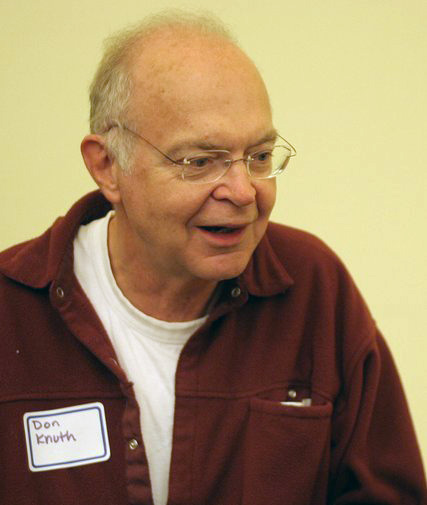
\includegraphics[width=\textwidth]{img/oef1-01}
      \caption{Donald Knuth, author of {\TeX}}
      \label{fig:don}
    \end{figure}

  \end{columns}

\end{frame}

\subsection{Tables}

\begin{frame}[fragile]
  \frametitle{Tables}
  
 \begin{columns}[c]
  \column{.6\textwidth}
  \small
\begin{semiverbatim}
\alert<1>{\\begin\{table\}}
  \alert<3>{\\begin\{tabular\}\{\alert<4>{l||c|r}\}}
  \alert<4>{\\hline}
  cel11 \alert<5>{&} 
    \alert<7>{\\multicolumn\{2\}\{c\}\{cel12\}} \alert<6>{\\\\}
  \alert<4>{\\hline \\hline}
  cel21 \alert<5>{&} cel22 \alert<5>{&} 
    \alert<7>{\\multirow\{2\}\{*\}\{cel23\}} \alert<6>{\\\\}
  cel31 \alert<5>{&} cel32 \alert<5>{&} \alert<6>{\\\\}
  \alert<3>{\\end\{tabular\}}
  \alert<2>{\\caption\{An example of 
    the capabilities of tables\}
  \\label\{tab:vb_table\}}
\alert<1>{\\end\{table\}}
\end{semiverbatim}

  \column{.4\textwidth}
    \begin{table}
      \begin{tabular}{l||c|r}
      \hline
      cel11 & \multicolumn{2}{c}{cel12} \\
      \hline \hline
      cel21 & cel22 & \multirow{2}{*}{cel23} \\
      cel31 & cel32 & \\
      \end{tabular}
      \caption{An example of the capabilities of tables}
      \label{tab:vb_table}
    \end{table}
  
  \end{columns}
\end{frame}

\subsection{Source code}

\begin{frame}[fragile]
  \frametitle{Inserting source code: simple}

\begin{semiverbatim}
\alert{\\begin\{verbatim\}}
public class MyApp \{
  public static void main(String args[]) \{
    System.out.println("Hello World");
  \}
\}
\alert{\\end\{verbatim\}}
\end{semiverbatim}
$\Rightarrow$
\begin{verbatim}
public class MyApp {
  public static void main(String args[]) {
    System.out.println("Hello World");
  }
}
\end{verbatim}  

\end{frame}

\begin{frame}[fragile]
  \frametitle{Inserting source code: \texttt{\textbackslash{}usepackage\{listings\}}}

\begin{semiverbatim}
\\lstset\{\%
  language=java,    breaklines=true,
  numbers=left,     frame=single,
  caption=\{My first Java program.\},
  label=code:helloworld
\}

\alert{\\begin\{lstlisting\}}
public class MyApp \{
  public static void main(String args[]) \{
    System.out.println("Hello World");
  \}
\}
\alert{\\end\{lstlisting\}}
\end{semiverbatim}

\end{frame}

\begin{frame}[fragile]
  \frametitle{Inserting source code: \texttt{\textbackslash{}usepackage\{listings\}}}

  \lstset{%
  language=java,    breaklines=true,
  numbers=left,     frame=single,
  caption={My first Java program.},
  label=code:helloworld
}

\begin{lstlisting}
public class MyApp {
  public static void main(String args[]) {
    System.out.println("Hello World");
  }
}
\end{lstlisting}

\end{frame}

\subsection{Bibliography}

\begin{frame}[fragile]
  \frametitle{Bibliography}

  \begin{itemize}
  \item<+-> The bibliography is an important part of a thesis
  \item<+-> Strict rules for layout (HoGent: APA-style)
  \item<+-> Only \emph{publications} are allowed
  \item<+-> Only sources that are referenced from the text
  \item<+-> {\LaTeX}, specifically Bib{\LaTeX} helps:
    \begin{itemize}
    \item<+-> ``bibliographic data base'' (in text format)
    \item<+-> Automatic layout, sorting
    \item<+-> Citations in the text (e.g.~\verb|\textcite{}|)
    \item<+-> Support through external tools (e.g. JabRef, Mendeley Desktop)
    \end{itemize}
  \end{itemize}
\end{frame}

\begin{frame}[fragile]
  \frametitle{Bibliography}

Example Bib{\LaTeX}-file content (*.bib):

\begin{semiverbatim}
\alert<2>{@book}\{\alert<4>{Knuth1998},
 \alert<3>{author} = \{Knuth, Donald E.\},
 \alert<3>{title} = \{The art of computer programming,  volume 3:
   sorting and searching\},
 \alert<3>{year} = \{1998\},
 publisher = \{Addison Wesley\},
 address = \{Redwood City, CA, USA\}
\} 
\end{semiverbatim}

\only<2>{Or: article, inproceedings, inbook, phdthesis, misc, \ldots}
\only<3>{Some fields are mandatory, depending op publication type}
\only<4>{Citations in the text:
  \begin{itemize}
     \item \alert{\texttt{\textbackslash{}textcite\{Knuth1998\}}} $\Rightarrow$ \textcite{Knuth1998}
    \item \alert{\texttt{\textbackslash{}autocite\{Knuth1998\}}} $\Rightarrow$ \autocite{Knuth1998}
  \end{itemize}
}

\end{frame}

\begin{frame}[fragile]
  \frametitle{Bibliography}

Inserting the bibliography
\begin{semiverbatim}
\\usepackage[backend=bibtex]\{biblatex\} \% Preamble
\\DeclareLanguageMapping\{english\}\{english-apa\}
\\addbibresource\{<database>\}
\dots
Citations in the text~\\textcite\{label\}.
\ldots
\\printbibliography
\end{semiverbatim}

$\Rightarrow$

\printbibliography

\end{frame}

\begin{frame}
  \frametitle{Bibliography}

  Short texts: typically numbered, according to occurrence in the text (e.g. article)
  \begin{center}
  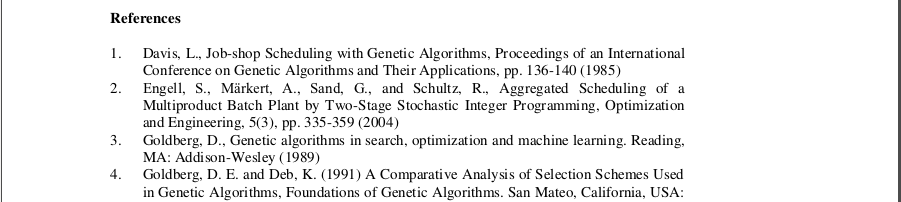
\includegraphics[width=.7\textwidth]{img/oef1-07}
  \end{center}

  Longer texts: names, alphabetically (e.g. report, book)
  \begin{center}
  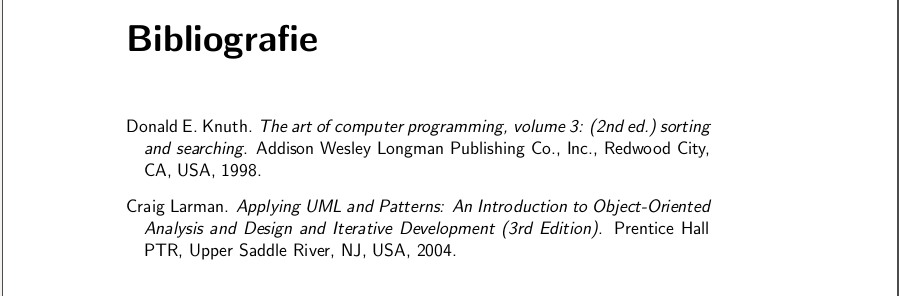
\includegraphics[width=.7\textwidth]{img/oef1-08}
  \end{center}

  \brightbox{HoGent uses the ``APA''-style \url{https://bib.hogent.be/how-to/bronnen-vermelden/refereren-volgens-apa6th/}}

\end{frame}

\section{Finally}

\begin{frame}
  \frametitle{Finally}
  
  \begin{itemize}
  \item Outside the scope of this presentation:
    \begin{itemize}
    \item<+-> Mathematical formulas, e.g.
    \begin{semiverbatim}
    \$x=-\\frac\{b \\pm \\sqrt\{b\^{}2 - 4ac\}\}\{2a\}\$
    \end{semiverbatim}
    $x=-\frac{b \pm \sqrt{b^2 - 4ac}}{2a}$
    \item<+-> Hundreds of packages (RTFM, Google is your friend)
    \item<+-> Presentations with Beamer (start e.g. with template from \url{https://github.com/bertvv/hogent-latex-sjablonen}

    \end{itemize}
  \item<+-> Need help? After trying yourself, contact \texttt{bert.vanvreckem@hogent.be}
  \end{itemize}
\end{frame}

\end{document}
